% =====================================================================
%  Mothbox : paramétrer sa Mothbox avec un téléphone (version paysage)
%  Compilation : pdfLaTeX
% =====================================================================
\documentclass[11pt,a4paper,openany]{report}
% =====================================================================
%  Préambule — compatible pdfLaTeX (Overleaf par défaut), XeLaTeX et LuaLaTeX
% =====================================================================
\usepackage{iftex}
\ifPDFTeX
  \usepackage[T1]{fontenc}
  \usepackage[utf8]{inputenc}
\fi
\usepackage{amsmath}
\usepackage[french]{babel}
\usepackage{libertinus}
\usepackage{microtype}

\usepackage[a4paper,top=2.5cm,bottom=2.5cm,left=2.4cm,right=2.4cm,headheight=14pt]{geometry}
\usepackage[table]{xcolor}
\usepackage{graphicx}

\usepackage[locale=FR,per-mode=symbol,group-minimum-digits=4]{siunitx}
\sisetup{range-phrase={\,\text{à}\,},list-final-separator={ et },inter-unit-product=\ensuremath{\cdot}}

\usepackage{booktabs}
\usepackage{tabularx}
\usepackage{longtable}
\usepackage{multirow}
\usepackage{array}
\usepackage{makecell}
\usepackage{caption}
\usepackage{subcaption}
\usepackage{float}
\usepackage{enumitem}
\usepackage{pdflscape}
\usepackage{eso-pic}

\usepackage{pifont}
\usepackage{tikz}
\usetikzlibrary{babel}
\usetikzlibrary{arrows.meta,positioning,fit,calc}

\usepackage[most]{tcolorbox}
\usepackage{listings}
\usepackage{fancyhdr}
\usepackage{titlesec}
\usepackage[hidelinks]{hyperref}
\usepackage[french,nameinlink]{cleveref}

% ---------------------------------------------------------------------
%  Couleurs
% ---------------------------------------------------------------------
\definecolor{pslbleu}{HTML}{1F4E8C}
\definecolor{pslbleuclair}{HTML}{E8EEF7}
\definecolor{pslorange}{HTML}{E8781A}
\definecolor{pslorangeclair}{HTML}{FDF0E4}
\definecolor{pslvert}{HTML}{2E7D4F}
\definecolor{pslvertclair}{HTML}{E7F3EC}
\definecolor{pslrouge}{HTML}{B3261E}
\definecolor{pslrougeclair}{HTML}{FBEAE9}
\definecolor{pslgris}{HTML}{5F6368}

\hypersetup{colorlinks=true,linkcolor=pslbleu,urlcolor=pslbleu,citecolor=pslbleu,
  pdftitle={OpenFlexure USB — Microscope en périphérique USB},
  pdfauthor={Tom Penfornis},pdfsubject={Liaison USB gadget et mise à l'heure}}

% ---------------------------------------------------------------------
%  Titres et en-têtes
% ---------------------------------------------------------------------
\titleformat{\chapter}[display]
  {\normalfont\sffamily\color{pslbleu}}
  {\large\MakeUppercase{\chaptertitlename}~\thechapter}
  {4pt}
  {\Huge\bfseries}
  [\vspace{4pt}{\color{pslorange}\titlerule[1.5pt]}]
\titlespacing*{\chapter}{0pt}{-10pt}{24pt}
\titleformat{\section}{\normalfont\sffamily\Large\bfseries\color{pslbleu}}{\thesection}{0.8em}{}
\titleformat{\subsection}{\normalfont\sffamily\large\bfseries\color{pslbleu!85!black}}{\thesubsection}{0.8em}{}
\titleformat{\subsubsection}{\normalfont\sffamily\normalsize\bfseries}{\thesubsubsection}{0.8em}{}

\pagestyle{fancy}
\fancyhf{}
\fancyhead[L]{\small\sffamily\color{pslgris}OpenFlexure USB — Rapport technique}
\fancyhead[R]{\small\sffamily\color{pslgris}\nouppercase{\leftmark}}
\fancyfoot[C]{\small\sffamily\thepage}
\renewcommand{\headrulewidth}{0.4pt}
\renewcommand{\headrule}{{\color{pslbleu!40}\hrule height\headrulewidth width\headwidth\vskip-\headrulewidth}}
\fancypagestyle{plain}{\fancyhf{}\fancyfoot[C]{\small\sffamily\thepage}\renewcommand{\headrulewidth}{0pt}}

\setcounter{tocdepth}{2}
\setcounter{secnumdepth}{3}
\setlength{\parskip}{0.35em}
\setlist{itemsep=2pt,topsep=4pt}

\captionsetup{font=small,labelfont={bf,sf,color=pslbleu},format=hang,margin=10pt}
\captionsetup[table]{position=top}
\renewcommand{\arraystretch}{1.18}
\newcolumntype{L}{>{\raggedright\arraybackslash}X}
\newcolumntype{C}{>{\centering\arraybackslash}X}

% ---------------------------------------------------------------------
%  Encadrés
% ---------------------------------------------------------------------
\newtcolorbox{synthese}[1][Synthèse]{enhanced,breakable,colback=pslbleuclair,colframe=pslbleu,
  fonttitle=\sffamily\bfseries,title={#1},arc=2pt,boxrule=0.6pt,left=6pt,right=6pt}
\newtcolorbox{choix}[1][Choix retenu]{enhanced,breakable,colback=pslvertclair,colframe=pslvert,
  fonttitle=\sffamily\bfseries,title={#1},arc=2pt,boxrule=0.6pt,left=6pt,right=6pt}
\newtcolorbox{attention}[1][Point de vigilance]{enhanced,breakable,colback=pslrougeclair,colframe=pslrouge,
  fonttitle=\sffamily\bfseries,title={#1},arc=2pt,boxrule=0.6pt,left=6pt,right=6pt}
\newtcolorbox{calcul}[1][Calcul]{enhanced,breakable,colback=white,colframe=pslorange,
  fonttitle=\sffamily\bfseries,coltitle=black,colbacktitle=pslorangeclair,title={#1},arc=2pt,boxrule=0.6pt,left=6pt,right=6pt}

% ---------------------------------------------------------------------
%  Code
% ---------------------------------------------------------------------
\lstdefinestyle{psl}{basicstyle=\ttfamily\footnotesize,keywordstyle=\color{pslbleu},
  commentstyle=\color{pslgris}\itshape,stringstyle=\color{pslorange!80!black},numbers=left,
  numberstyle=\tiny\color{pslgris},frame=single,rulecolor=\color{pslbleu!30},backgroundcolor=\color{pslbleuclair!40},
  breaklines=true,columns=fullflexible,keepspaces=true,showstringspaces=false,
  literate={é}{{\'e}}1 {è}{{\`e}}1 {à}{{\`a}}1 {ç}{{\c{c}}}1 {ê}{{\^e}}1 {É}{{\'E}}1 {ô}{{\^o}}1 {î}{{\^i}}1 {û}{{\^u}}1 {ù}{{\`u}}1 {Ø}{{\O}}1 {×}{{$\times$}}1 {â}{{\^a}}1 {⇄}{{$\leftrightarrows$}}1 {→}{{$\rightarrow$}}1 {«}{{\guillemotleft}}1 {»}{{\guillemotright}}1 {À}{{\`A}}1}
\lstset{style=psl}

% ---------------------------------------------------------------------
%  Raccourcis
% ---------------------------------------------------------------------
\newcommand{\comp}[1]{\textsf{#1}}
\newcommand{\fichier}[1]{{\small\nolinkurl{#1}}}

% Pas de citation (lien dans un lien) dans les listes des figures et des tableaux
\let\listoffiguresorig\listoffigures
\let\listoftablesorig\listoftables
\renewcommand{\listoffigures}{\begingroup\renewcommand{\cite}[2][]{}\listoffiguresorig\endgroup}
\renewcommand{\listoftables}{\begingroup\renewcommand{\cite}[2][]{}\listoftablesorig\endgroup}
\crefname{lstlisting}{listing}{listings}
\Crefname{lstlisting}{Listing}{Listings}

\geometry{landscape,top=1.6cm,bottom=1.5cm,left=1.8cm,right=1.8cm,headheight=14pt}

\hypersetup{pdftitle={Paramétrer sa Mothbox avec un téléphone},
  pdfsubject={Guide de terrain Mothbox, version paysage}}
\fancyhf{}
\fancyhead[L]{\small\sffamily\color{pslgris}Mothbox, guide de terrain}
\fancyhead[R]{\small\sffamily\color{pslgris}\nouppercase{\rightmark}}
\fancyfoot[C]{\small\sffamily\thepage}
\graphicspath{{annotees/}}
\captionsetup{labelsep=colon}

\newcommand{\sw}[1]{\textsf{\bfseries #1}}
\newcommand{\on}{\textcolor{pslvert}{\textsf{\bfseries ON}}}
\newcommand{\off}{\textcolor{pslrouge}{\textsf{\bfseries OFF}}}
\newcommand{\pasc}[2]{\tikz[baseline=(n.base)]\node[circle,fill=#1,text=white,font=\sffamily\bfseries\footnotesize,inner sep=1.5pt,minimum size=1.2em](n){#2};}
\newcommand{\pas}[1]{\pasc{pslrouge}{#1}}
\newtcolorbox{astuce}[1][Bon réflexe]{enhanced,breakable,colback=pslvertclair,colframe=pslvert,
  fonttitle=\sffamily\bfseries,title={#1},arc=2pt,boxrule=0.6pt,left=6pt,right=6pt}

\newcommand{\fiche}[2]{%
  \clearpage
  \markright{#2}%
  \noindent{\sffamily\color{pslorange}\bfseries\large #1}\par\vspace{-2pt}
  \noindent{\sffamily\color{pslbleu}\bfseries\fontsize{24}{28}\selectfont #2}\par\vspace{2pt}
  \noindent{\color{pslorange}\rule{\textwidth}{1.5pt}}\par\vspace{8pt}}

\setlist{itemsep=3pt,topsep=3pt}

\begin{document}
\thispagestyle{empty}

% ---------------------------------------------------------------------
%  Page 1 : couverture et essentiel
% ---------------------------------------------------------------------
\begin{tikzpicture}[remember picture,overlay]
  \fill[pslvert] (current page.north west) rectangle ([xshift=11.5cm]current page.south west);
  \fill[pslorange] ([xshift=11.5cm]current page.north west) rectangle ([xshift=11.8cm]current page.south west);
  \node[anchor=north west,text=white!85!pslvert,font=\sffamily\small,inner sep=0pt] at ([xshift=1.6cm,yshift=-1.8cm]current page.north west) {Mothbox Pro, PSL3D};
  \node[anchor=north west,text=white,font=\sffamily\bfseries\fontsize{30}{36}\selectfont,inner sep=0pt,text width=8.6cm] at ([xshift=1.6cm,yshift=-2.7cm]current page.north west) {Paramétrer sa Mothbox avec un téléphone};
  \node[anchor=north west,text=white!90!pslvert,font=\sffamily\Large,inner sep=0pt,text width=8.4cm] at ([xshift=1.6cm,yshift=-8.4cm]current page.north west) {Deux switches, un wifi, une page web};
  \node[anchor=south west,text=white!90!pslvert,font=\sffamily\small,inner sep=0pt,text width=8.4cm] at ([xshift=1.6cm,yshift=1.6cm]current page.south west) {Tom Penfornis\\Version 1.0, 26 novembre 2026\\Image \texttt{5.2.1-webui}};
\end{tikzpicture}

\hspace*{10.4cm}\begin{minipage}[t]{15.0cm}
\vspace{0pt}
{\sffamily\color{pslbleu}\bfseries\fontsize{22}{26}\selectfont L'essentiel}\par
{\color{pslorange}\rule{\linewidth}{1.5pt}}\par\vspace{8pt}

\begin{synthese}[En bref]
Avant, pour régler une Mothbox, il fallait un ordinateur, le logiciel VNC, un identifiant et savoir quel fichier modifier.
Désormais, \textbf{un téléphone suffit} : la Mothbox crée son propre wifi et affiche une page qui guide pas à pas.
\end{synthese}

\begin{enumerate}[label=\protect\pas{\arabic*},leftmargin=2.2em,itemsep=7pt]
  \item Mettre les switches \sw{Active} et \sw{DEBUG} sur \on{}, puis brancher la batterie.
  \item Attendre 2 à 3 minutes, puis connecter le téléphone au wifi \texttt{Mothbox-…} (mot de passe \texttt{lunaluna}). La page s'ouvre toute seule.
  \item Suivre les 4 étapes de la page : \emph{Heure}, \emph{Planning}, \emph{Tester}, \emph{Terminer}.
  \item Remettre \sw{DEBUG} sur \off{} (laisser \sw{Active} sur \on{}) et appuyer sur \emph{Redémarrer maintenant}. C'est prêt.
\end{enumerate}

\begin{attention}[Lire un switch]
Un switch est sur \on{} quand son levier est poussé \textbf{du côté de l'inscription \og ON \fg{} du boîtier noir}. Sur la carte, elle est imprimée à l'envers et se lit \og NO \fg{} : c'est le côté \textbf{bas} sur toutes les photos. Le petit \og On \fg{} imprimé sur la carte verte est trompeur.
\end{attention}
\end{minipage}

% ---------------------------------------------------------------------
%  Page 2 : les switches
% ---------------------------------------------------------------------
\fiche{1}{Repérer les switches}

\begin{minipage}[t]{0.3\textwidth}
\vspace{0pt}\centering
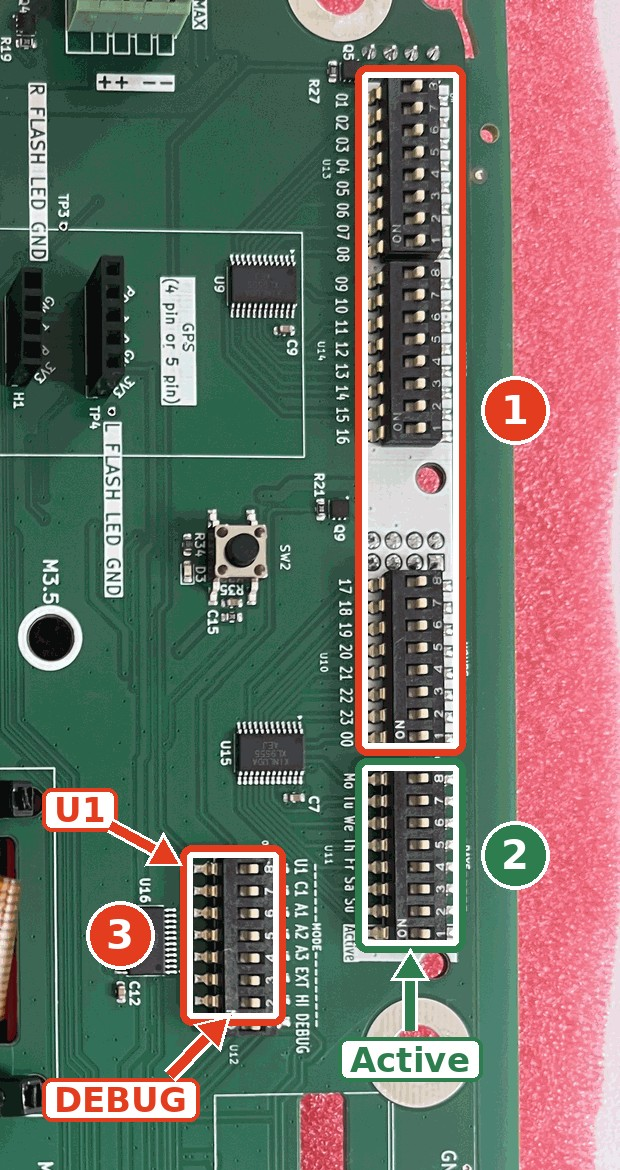
\includegraphics[height=13.4cm]{carte_reperes.jpg}
\end{minipage}\hfill
\begin{minipage}[t]{0.67\textwidth}
\vspace{0pt}
\begin{description}[leftmargin=0pt,itemsep=3pt]
  \item[\pas{1} Heures (01 à 00)] un switch par heure, utilisés seulement en mode manuel.
  \item[\pas{2} Jours + Active] les jours (Mo à Su) pour le mode manuel, et \sw{Active}, \textbf{le plus important}.
  \item[\pas{3} Mode] détaillés ci-dessous.
\end{description}
\vspace{4pt}
\begin{minipage}[t]{0.42\linewidth}
\vspace{0pt}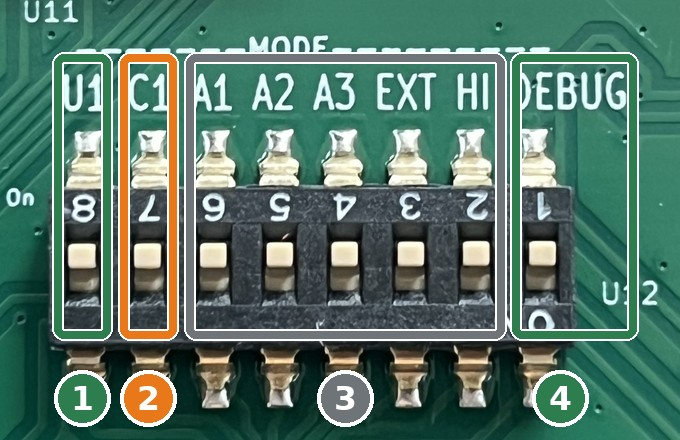
\includegraphics[width=\linewidth]{rangee_mode.jpg}
\end{minipage}\hfill
\begin{minipage}[t]{0.55\linewidth}
\vspace{0pt}\sffamily\small
\begin{tabularx}{\linewidth}{@{}c>{\raggedright\arraybackslash}p{1.5cm}L@{}}
\toprule
 & Switch & Rôle \\
\midrule
\pasc{pslvert}{1} & \sw{U1} & \textbf{Mode manuel} : planning réglé par les switches de la carte. \\
\pasc{pslorange}{2} & \sw{C1} & \textbf{Test des lumières} (avec \sw{DEBUG}) : toutes les voies clignotent en boucle. \\
\pasc{pslgris}{3} & \sw{A1} à \sw{HI} & \textbf{Réservés}, sans effet aujourd'hui. \\
\pasc{pslvert}{4} & \sw{DEBUG} & \textbf{Mode réglage} : wifi et page web. \\
\bottomrule
\end{tabularx}
\end{minipage}

\vspace{8pt}
\begin{astuce}[En pratique]
Laissez \sw{C1}, \sw{A1}, \sw{A2}, \sw{A3}, \sw{EXT} et \sw{HI} sur \off. \sw{C1} brouille les tests de la page s'il est sur \on.
\sw{A1} à \sw{A3} (voies d'attraction), \sw{EXT} (sortie externe) et \sw{HI} (alimentation secteur) sont prévus pour une version future du logiciel.
\end{astuce}
\end{minipage}

% ---------------------------------------------------------------------
%  Page 3 : les quatre positions
% ---------------------------------------------------------------------
\fiche{2}{Les quatre positions à connaître}

Les switches ne sont lus qu'\textbf{au démarrage} : après un changement, il faut redémarrer (débrancher puis rebrancher, ou utiliser le bouton de la page).
\vspace{6pt}

\newcommand{\cas}[4]{%
\begin{minipage}[t]{0.235\textwidth}\centering
\includegraphics[width=\linewidth]{#1}\par\vspace{4pt}
{\sffamily\bfseries\color{#2}#3}\par\vspace{2pt}
{\small #4}
\end{minipage}}
\noindent
\cas{pos_tout_off.jpg}{pslgris}{Rangement, transport, charge}{\sw{Active} \off, \sw{DEBUG} \off.\\La Mothbox s'éteint aussitôt qu'elle se réveille.}\hfill
\cas{pos_active_debug.jpg}{pslbleu}{Réglage avec le téléphone}{\sw{Active} \on, \sw{DEBUG} \on.\\Wifi et page web, aucune capture.}\hfill
\cas{pos_active_seul.jpg}{pslvert}{En service}{\sw{Active} \on, \sw{DEBUG} \off.\\Elle dort et se réveille aux heures prévues.}\hfill
\cas{pos_debug_sans_active.jpg}{pslrouge}{À éviter}{\sw{Active} \off, \sw{DEBUG} \on.\\\sw{Active} prime : elle s'éteint, pas de wifi.}

\vspace{8pt}
{\small\color{pslgris} Anneau vert : switch sur \on. Anneau rouge : switch sur \off.}

% ---------------------------------------------------------------------
%  Page 4 : se connecter + étape 1
% ---------------------------------------------------------------------
\fiche{3}{Se connecter, puis régler l'heure}

\begin{minipage}[t]{0.44\textwidth}
\vspace{0pt}
{\sffamily\bfseries\color{pslbleu}Se connecter}
\begin{enumerate}[label=\protect\pas{\arabic*},leftmargin=2.2em,itemsep=5pt]
  \item \sw{Active} et \sw{DEBUG} sur \on, puis brancher la batterie.
  \item Attendre \textbf{2 à 3 minutes}.
  \item Sur le téléphone, choisir le wifi \texttt{Mothbox-} suivi du nom de la boîte. Mot de passe : \texttt{lunaluna}.
  \item La page s'ouvre toute seule. Sinon, taper \texttt{192.168.50.5} dans le navigateur.
\end{enumerate}
\begin{astuce}[\og Pas d'accès Internet \fg{}]
C'est normal. Choisir \emph{Rester connecté}.
\end{astuce}
La page est en français ou en anglais (bouton \textsf{EN}/\textsf{FR} en haut à droite).
\end{minipage}\hfill
\begin{minipage}[t]{0.24\textwidth}
\vspace{0pt}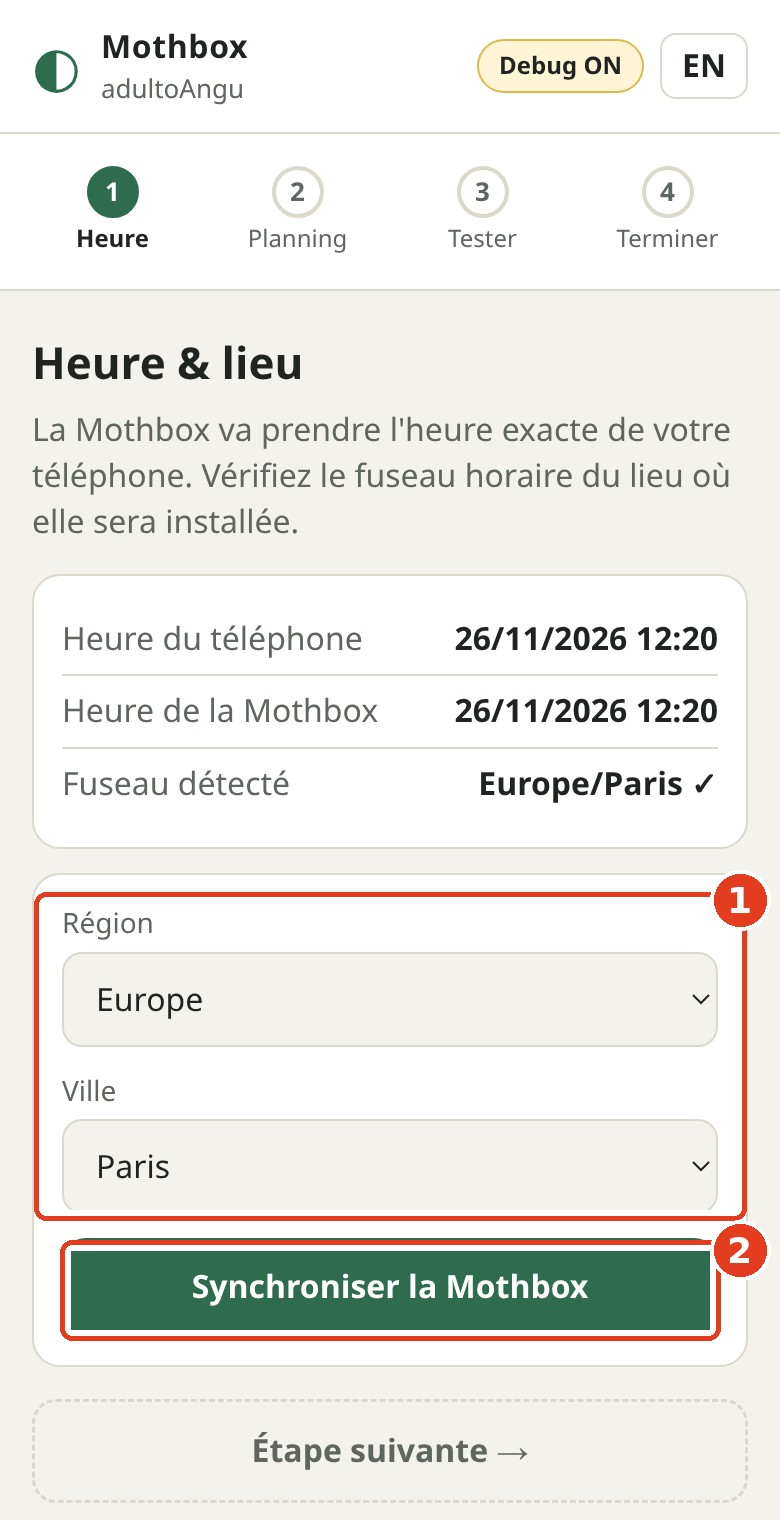
\includegraphics[width=\linewidth]{ecran_etape1.jpg}
\end{minipage}\hfill
\begin{minipage}[t]{0.27\textwidth}
\vspace{0pt}
{\sffamily\bfseries\color{pslbleu}Étape 1 : Heure et lieu}\par\vspace{4pt}
La Mothbox prend l'heure du téléphone.
\begin{description}[leftmargin=0pt,itemsep=5pt]
  \item[\pas{1}] Vérifier le fuseau horaire ; le changer si le téléphone est réglé sur un autre pays.
  \item[\pas{2}] Appuyer sur \emph{Synchroniser la Mothbox}.
\end{description}
\end{minipage}

% ---------------------------------------------------------------------
%  Page 5 : étapes 2 et 3
% ---------------------------------------------------------------------
\fiche{4}{Choisir le planning, puis tester}

\begin{minipage}[t]{0.22\textwidth}
\vspace{0pt}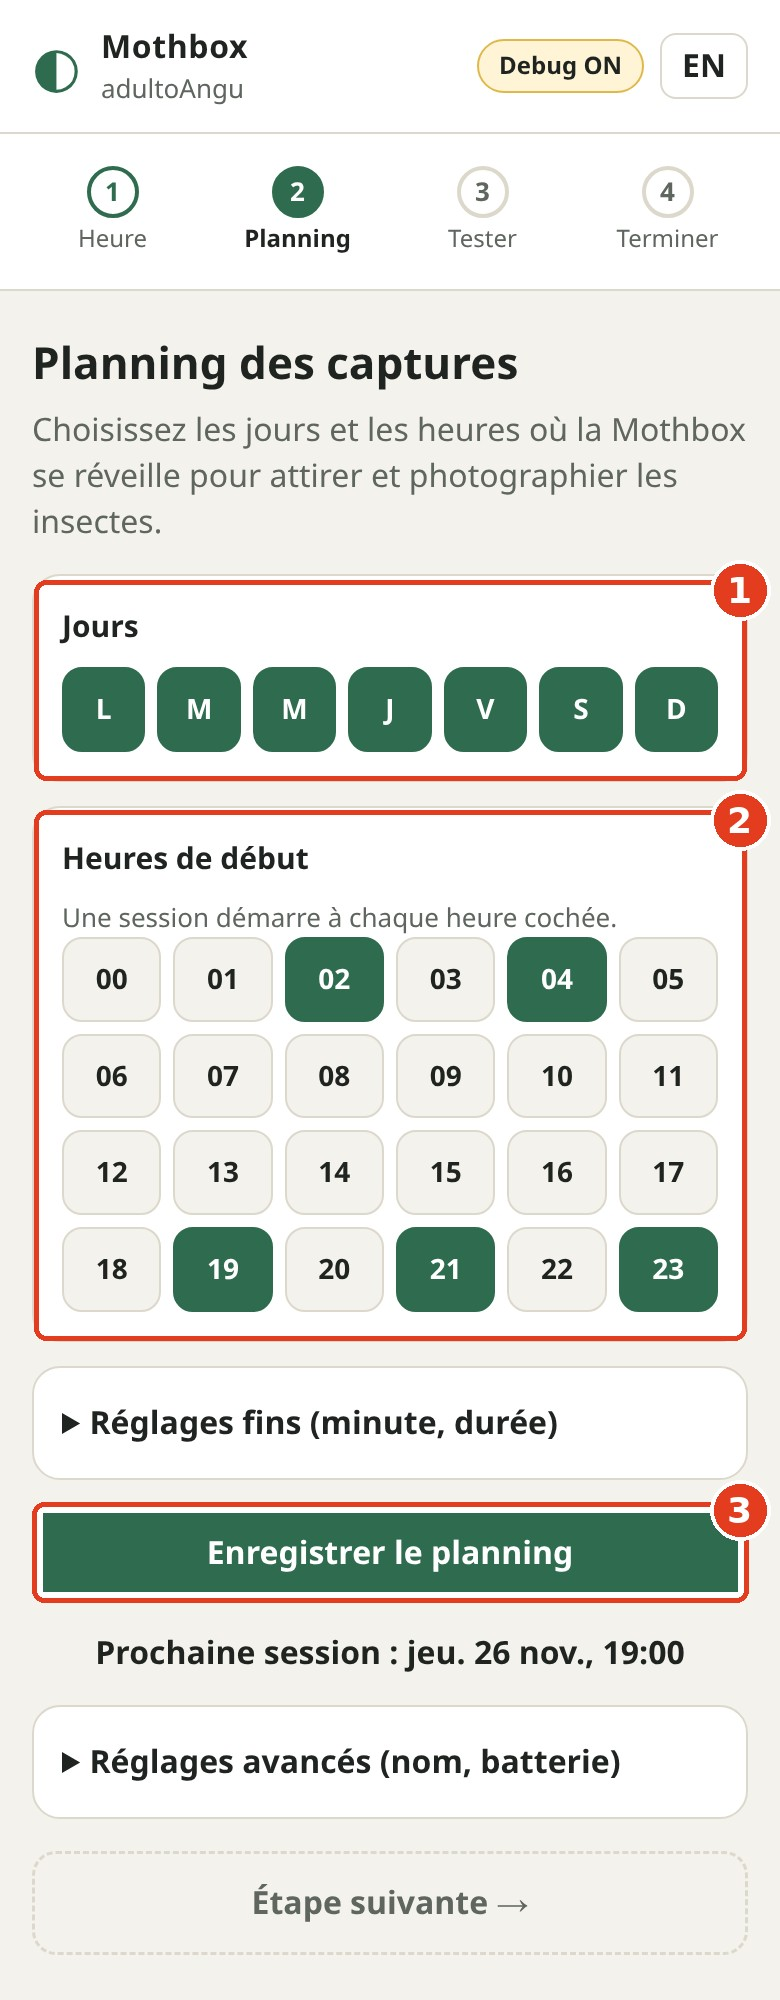
\includegraphics[width=\linewidth]{ecran_etape2.jpg}
\end{minipage}\hfill
\begin{minipage}[t]{0.26\textwidth}
\vspace{0pt}
{\sffamily\bfseries\color{pslbleu}Étape 2 : Planning}\par\vspace{4pt}
\begin{description}[leftmargin=0pt,itemsep=5pt]
  \item[\pas{1}] Les jours de capture.
  \item[\pas{2}] Les heures de début : une session démarre à chaque heure cochée.
  \item[\pas{3}] \emph{Enregistrer le planning}.
\end{description}
\small\emph{Réglages fins} : minute de départ et durée. \emph{Réglages avancés} : nom et batterie.
\end{minipage}\hfill
\begin{minipage}[t]{0.22\textwidth}
\vspace{0pt}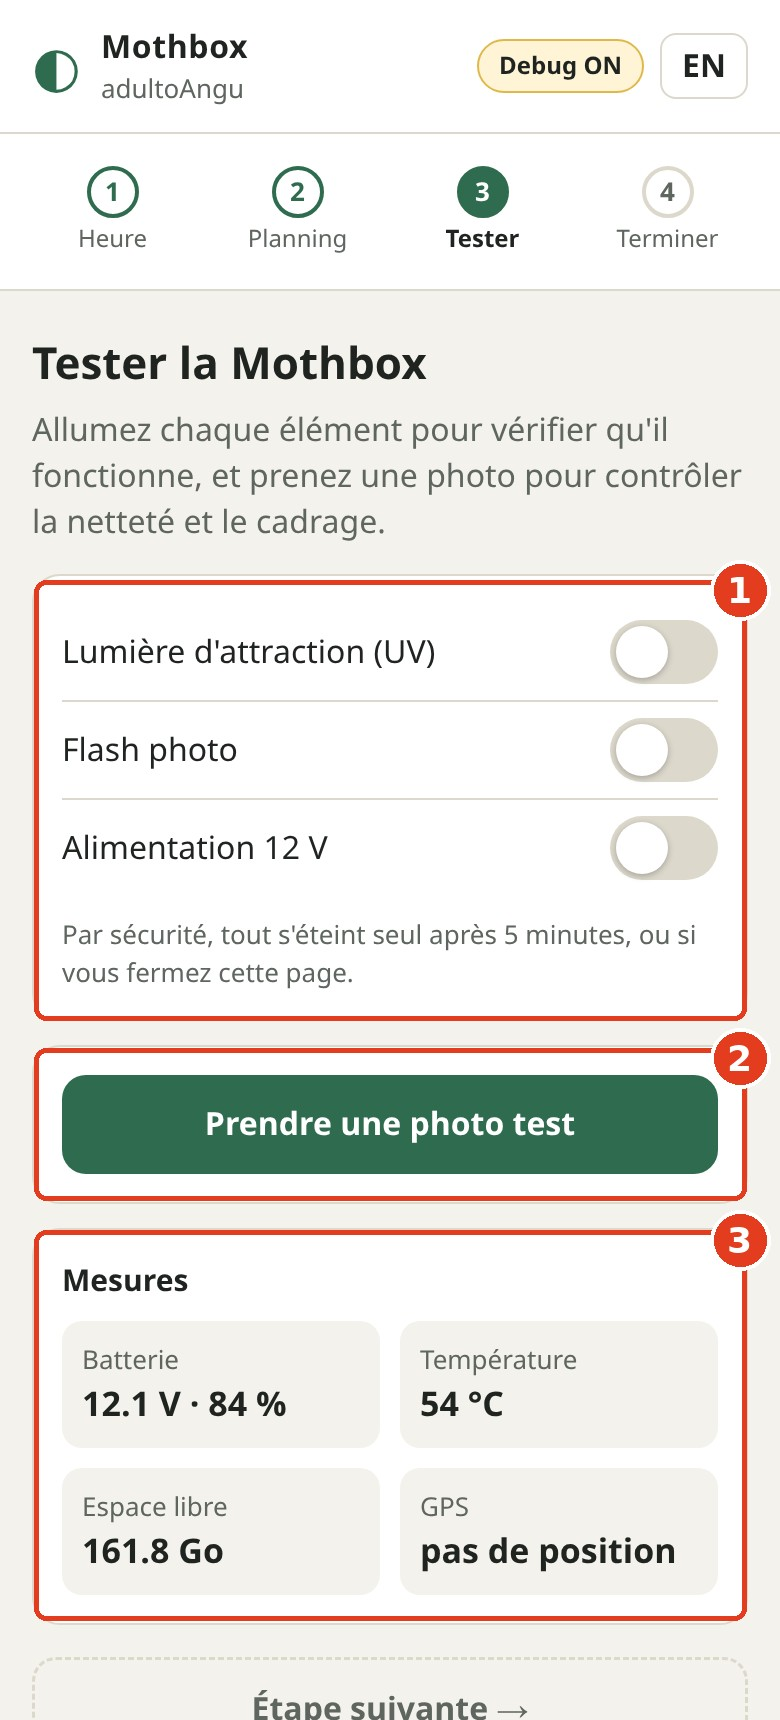
\includegraphics[width=\linewidth]{ecran_etape3.jpg}
\end{minipage}\hfill
\begin{minipage}[t]{0.25\textwidth}
\vspace{0pt}
{\sffamily\bfseries\color{pslbleu}Étape 3 : Tester}\par\vspace{4pt}
\begin{description}[leftmargin=0pt,itemsep=5pt]
  \item[\pas{1}] Allumer la lumière UV, le flash, le 12\,V.
  \item[\pas{2}] Prendre une photo test : le drap doit être net et remplir l'image.
  \item[\pas{3}] Lire les mesures : batterie, température, espace libre, GPS.
\end{description}
\small Tout s'éteint seul après 5 minutes, ou si la page est fermée.
\end{minipage}

% ---------------------------------------------------------------------
%  Page 6 : étape 4
% ---------------------------------------------------------------------
\fiche{5}{Mettre en service}

\begin{minipage}[t]{0.22\textwidth}
\vspace{0pt}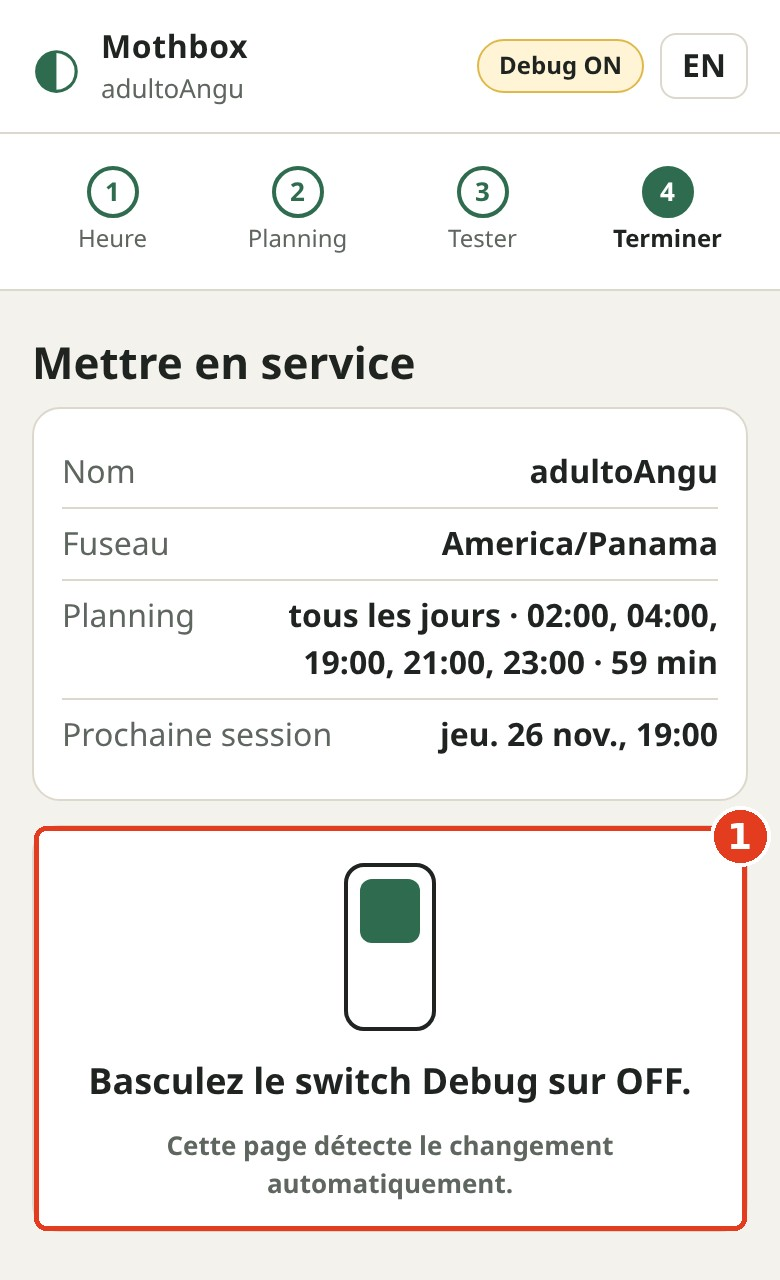
\includegraphics[width=\linewidth]{ecran_etape4.jpg}
\end{minipage}\hfill
\begin{minipage}[t]{0.22\textwidth}
\vspace{0pt}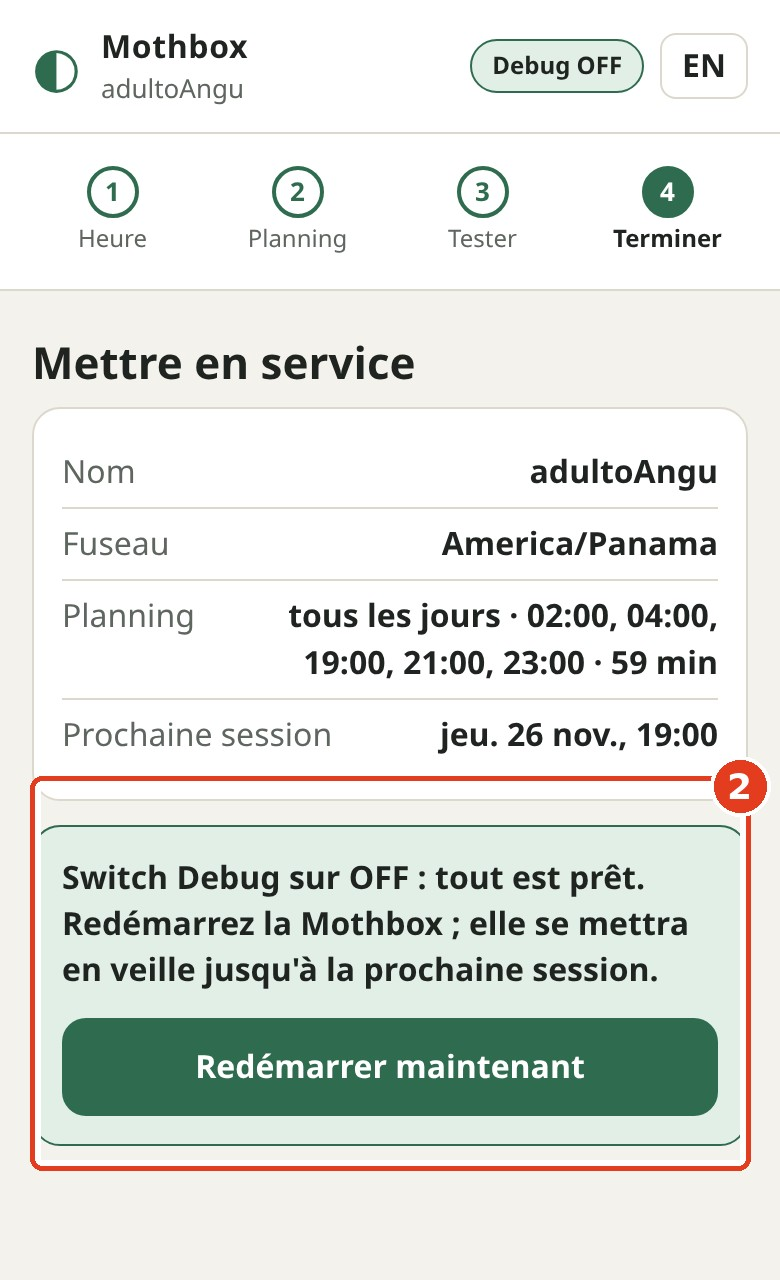
\includegraphics[width=\linewidth]{ecran_etape4_pret.jpg}
\end{minipage}\hfill
\begin{minipage}[t]{0.5\textwidth}
\vspace{0pt}
Un récapitulatif rappelle le nom, le fuseau, le planning et la prochaine session.
\begin{description}[leftmargin=0pt,itemsep=6pt]
  \item[\pas{1} Basculer DEBUG sur OFF] directement sur la carte, sans débrancher. \textbf{Laisser Active sur ON.} La page le détecte en quelques secondes.
  \item[\pas{2} Redémarrer maintenant] La Mothbox coupe son wifi et dort jusqu'à la prochaine session. La page peut être fermée.
\end{description}
\begin{attention}[La page affiche \og le switch Active est sur OFF \fg{}]
Remettre \sw{Active} sur \on{} : sinon la Mothbox s'éteindrait à chaque réveil sans prendre une seule photo.
\end{attention}
\end{minipage}

% ---------------------------------------------------------------------
%  Page 7 : mode manuel + dépannage
% ---------------------------------------------------------------------
\fiche{6}{Mode manuel et dépannage}

\begin{minipage}[t]{0.2\textwidth}
\vspace{0pt}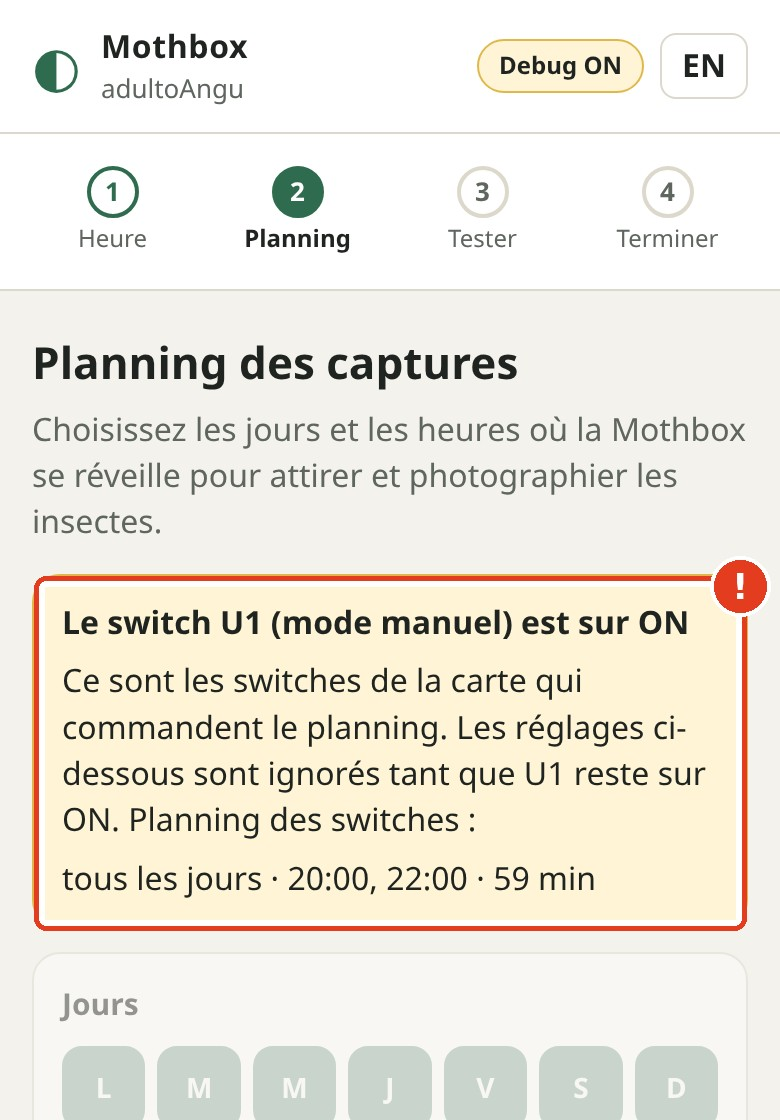
\includegraphics[width=\linewidth]{ecran_etape2_u1.jpg}
\end{minipage}\hfill
\begin{minipage}[t]{0.3\textwidth}
\vspace{0pt}
{\sffamily\bfseries\color{pslbleu}Mode manuel, sans téléphone}
\begin{enumerate}[label=\protect\pas{\arabic*},leftmargin=2.2em,itemsep=4pt]
  \item \sw{U1} sur \on.
  \item Les heures et les jours voulus sur \on.
  \item Redémarrer.
\end{enumerate}
\small Les switches priment alors sur la page (bandeau jaune). Chaque session démarre à l'heure pile et dure 59 minutes.
\end{minipage}\hfill
\begin{minipage}[t]{0.45\textwidth}
\vspace{0pt}
{\sffamily\bfseries\color{pslbleu}En cas de problème}\par\vspace{4pt}
\sffamily\footnotesize
\begin{tabularx}{\linewidth}{@{}>{\raggedright\arraybackslash}p{3.3cm}L@{}}
\toprule
Constat & À essayer \\
\midrule
Pas de wifi \texttt{Mothbox-…} & Attendre 3 min ; \sw{Active} \textbf{et} \sw{DEBUG} sur \on ; redémarrer ; chercher aussi \texttt{mothboxwifi}. \\
La page ne s'ouvre pas & Taper \texttt{192.168.50.5}. \\
Le téléphone se déconnecte & Choisir \emph{Rester connecté} ; couper les données mobiles. \\
\og La carte n'a pas répondu \fg{} & Vérifier les branchements lumière et flash. \\
\og La caméra n'a pas répondu \fg{} & Vérifier la nappe de la caméra. \\
Photos aux mauvaises heures & Refaire l'étape 1 ; \sw{U1} sur \off{} si le planning vient de la page. \\
Aucune photo & \sw{Active} sur \on, \sw{DEBUG} sur \off. \\
\bottomrule
\end{tabularx}
\end{minipage}

% ---------------------------------------------------------------------
%  Page 8 : préparer une carte SD
% ---------------------------------------------------------------------
\fiche{7}{Pour l'équipe : préparer une carte SD}

\begin{minipage}[t]{0.55\textwidth}
\vspace{0pt}
Tout se fait avec \textbf{Raspberry Pi Imager}, gratuit (Windows, macOS, Linux : \texttt{raspberrypi.com/software}). Aucune commande à taper.

Fichier : \fichier{mothbox_Pro_Pi5_v5.2.1-webui_2026-11-26.img.xz} (\texttt{github.com/Tom-PSLD/mothbox-webui/releases}), \textbf{à ne pas décompresser}.
\begin{enumerate}[label=\protect\pas{\arabic*},leftmargin=2.2em,itemsep=5pt]
  \item Insérer la carte SD (16\,Go minimum).
  \item \emph{Appareil} : \textbf{Raspberry Pi 5}.
  \item \emph{Système d'exploitation} : tout en bas, \textbf{Utiliser une image personnalisée}, puis le \fichier{.img.xz}.
  \item \emph{Stockage} : la carte SD (vérifier sa taille, elle sera effacée).
  \item Personnalisation de l'OS : répondre \textbf{Non}.
  \item Attendre la fin (environ 10 minutes), retirer la carte et la mettre dans la Mothbox.
\end{enumerate}
\end{minipage}\hfill
\begin{minipage}[t]{0.4\textwidth}
\vspace{0pt}
\begin{attention}[Ne pas personnaliser l'OS]
Si Raspberry Pi Imager propose de régler un nom d'utilisateur, un mot de passe ou un wifi, refuser : la Mothbox pourrait ne plus créer son propre wifi.
\end{attention}
\begin{astuce}[Ce que contient l'image]
Le système Mothbox 5.2.1 d'origine, la page de réglage, et aucun wifi enregistré.
\end{astuce}
\end{minipage}

\end{document}
